\documentclass[border=10pt]{standalone}

\usepackage{tikz}
\usepackage{tikzsymbols}
\usetikzlibrary{calc,patterns,shapes.geometric}

\def\centerarc[#1](#2)(#3:#4:#5){\draw[#1] ($(#2)+({#5*cos(#3)},{#5*sin(#3)})$) arc (#3:#4:#5);}

\begin{document}
	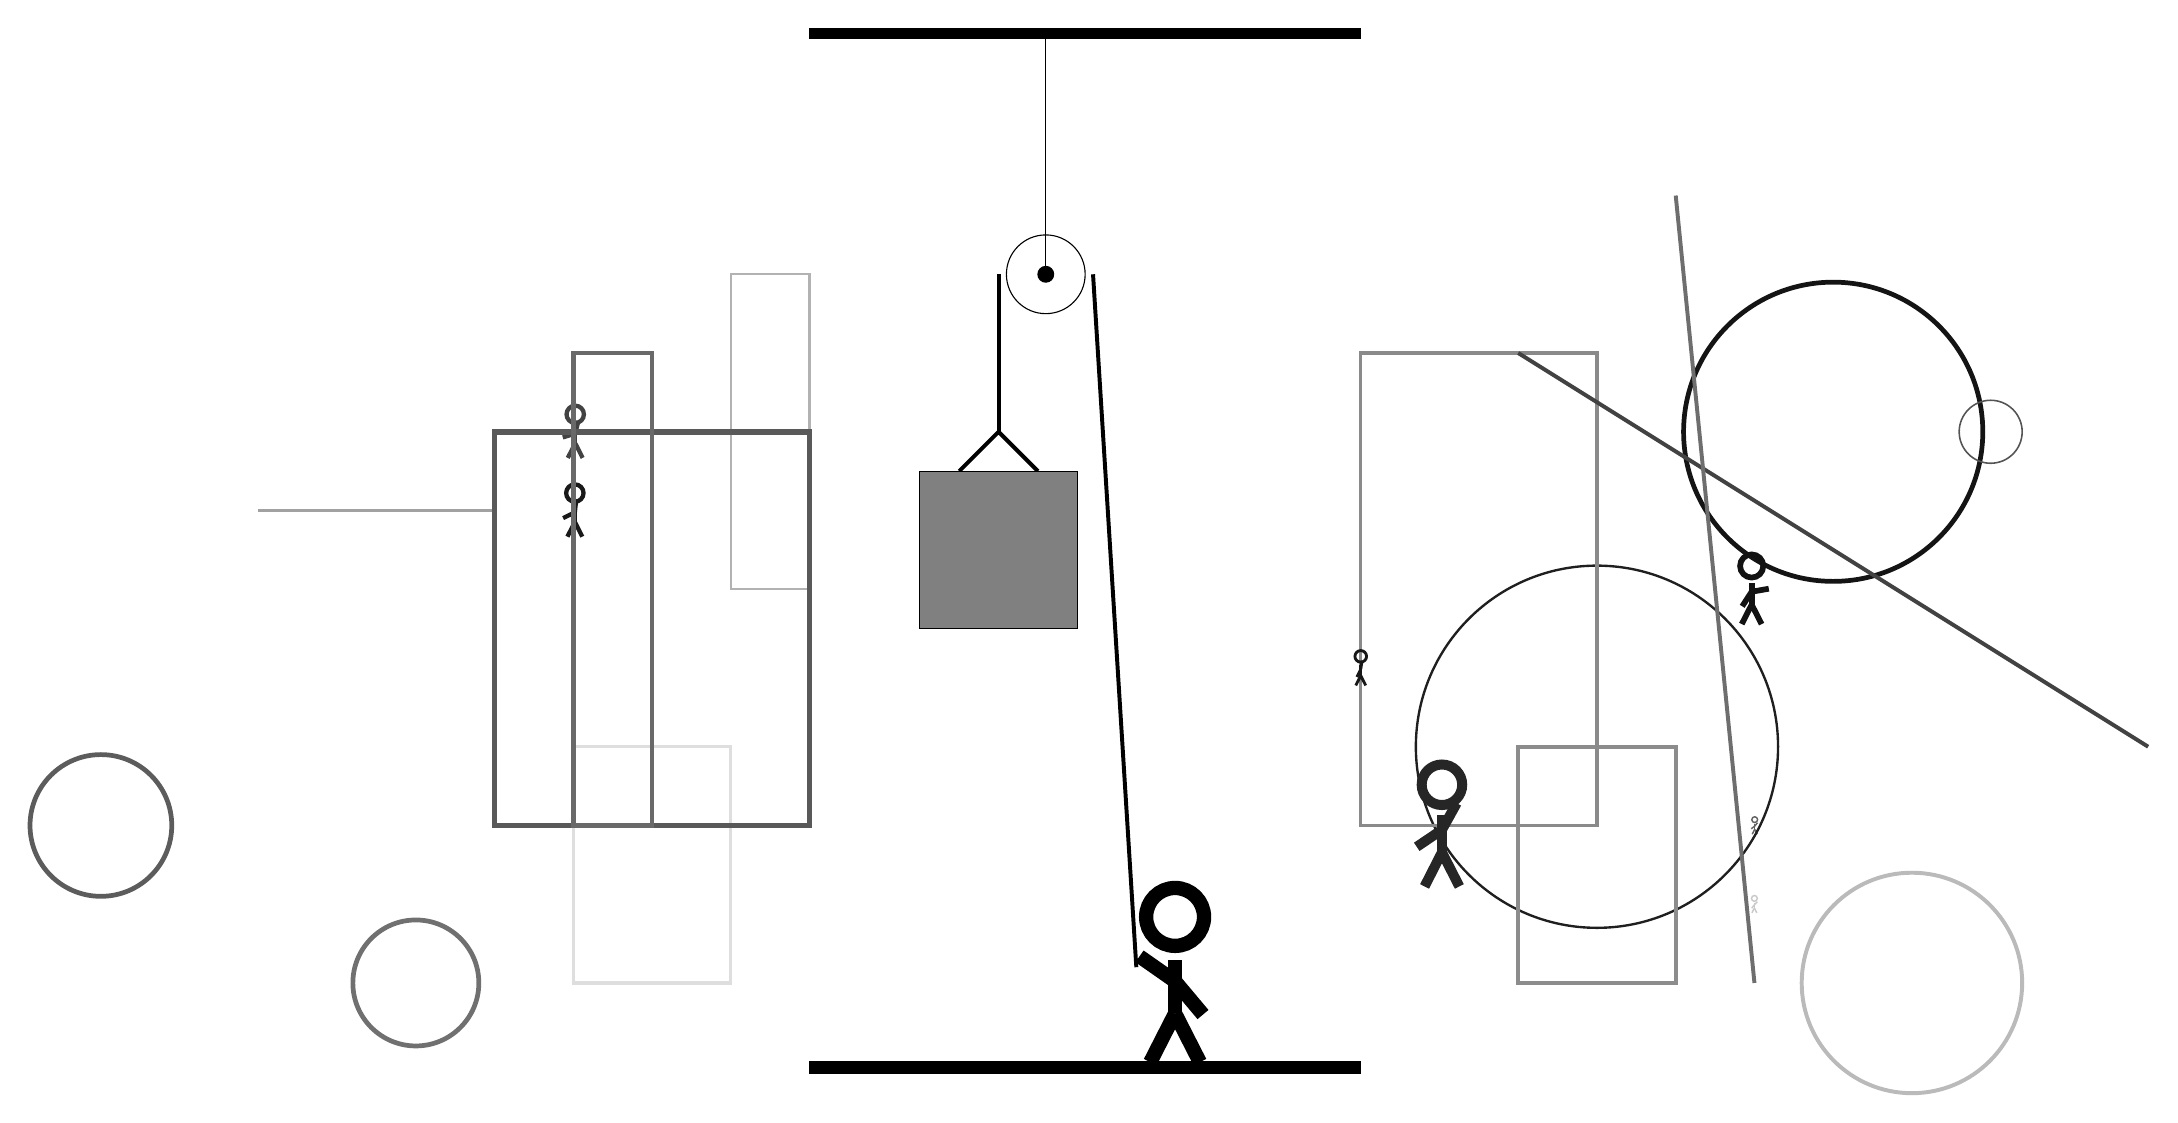
\begin{tikzpicture}
		%%%%% START %%%%%
		
		\draw[fill=black] (-2, 10) rectangle (5, 10.125);
		
		\draw (1, 7) circle (0.5);
		\draw[fill=black] (1, 7) circle (0.1);
		\draw (1, 10) -- (1, 7);
		
		\draw[line width=0.5mm] (-0.1, 4.5) -- (0.4, 5.0) -- (0.9, 4.5);
		\draw[fill=black!50] (-0.6, 4.5) rectangle (1.4, 2.5);
		
		\draw[line width=0.5mm] (0.4, 7) -- (0.4, 5.0);
		\centerarc[line width=0.5mm](1, 7)(0:180:0.6);
		\draw[line width=0.5mm](1.6, 7) -- (2.15, -1.8);
		
		\node at (2.6, -1.9) {\Strichmaxerl[10][-35][-50]};
		
		\draw [line width=0.6mm, color=black!64](-11, 0) circle (0.9);
		
		\draw[line width=0.5mm, color=black!37](-6, 4) -- (-9, 4);
		\node[line width=0.7mm, color=black!61] at (10, 0) {\Strichmaxerl[1][38][50]};
		\node[line width=0.3mm, color=black!74] at (-5, 5) {\Strichmaxerl[3][17][76]};
		
		\draw [line width=0.6mm, color=black!92](11, 5) circle (1.9);
		\draw [line width=0.3mm, color=black!88](8, 1) circle (2.3);
		
		\draw[line width=0.5mm, color=black!45] (7, 1) rectangle (9, -2);
		
		\draw[line width=0.4mm, color=black!13] (-3, 1) rectangle (-5, -2);
		\node[line width=0.4mm, color=black!90] at (-5, 4) {\Strichmaxerl[3][26][84]};
		\draw[line width=0.3mm, color=black!30] (-2, 7) rectangle (-3, 3);
		\draw[line width=0.4mm, color=black!46] (5, 0) rectangle (8, 6);
		\draw[line width=0.5mm, color=black!74](7, 6) -- (15, 1);
		\draw [line width=0.6mm, color=black!56](-7, -2) circle (0.8);
		\draw[line width=0.7mm, color=black!65] (-2, 0) rectangle (-6, 5);
		\draw[line width=0.5mm, color=black!57](10, -2) -- (9, 8);
		\node[line width=0.4mm, color=black!93] at (10, 3) {\Strichmaxerl[4][57][10]};
		\draw [line width=0.5mm, color=black!27](12, -2) circle (1.4);
		\draw[line width=0.6mm, color=black!59] (-4, 6) rectangle (-5, 0);
		\node[line width=0.3mm, color=black!21] at (10, -1) {\Strichmaxerl[1][51][47]};
		\node[line width=0.7mm, color=black!91] at (5, 2) {\Strichmaxerl[2][64][81]};
		\draw [line width=0.2mm, color=black!67](13, 5) circle (0.4);
		
		\node[line width=0.2mm, color=black!85] at (6, 0) {\Strichmaxerl[7][34][61]};
		
		\draw[fill=black] (-2, -3) rectangle (5, -3.15);
		
		%%%%% END %%%%%
	\end{tikzpicture}
\end{document}